% ex: ts=2 sw=2 sts=2 et filetype=tex
% SPDX-License-Identifier: CC-BY-SA-4.0

\documentclass[12pt,addpoints]{exam}

\usepackage[utf8]{inputenc}
\usepackage[T1]{fontenc}
%\usepackage[spanish]{babel}
\usepackage[letterpaper]{geometry}
\usepackage{graphicx}
%\usepackage{multicol}
%\setlength{\columnsep}{2cm}
%\usepackage{amssymb}

\pagestyle{headandfoot}
\headrule
\header{Pensamiento matemático II}{Examen Parcial II}{CBTIS 246}
\footer{}{Página \thepage\ de \numpages}{}

\pointpoints{punto}{puntos}
\renewcommand{\solutiontitle}{\textbf{Solución: }}

%\printanswers

\begin{document}
%\begin{center}
%\fbox{\fbox{\parbox{5.5in}{\centering
%Lee con atención cada pregunta y responde en
%el espacio ubicado en la parte izquierda.
%}}}
%\end{center}
%
%\vspace{5mm}

Nombre:\enspace\hrulefill

\vspace{5mm}

Grupo:\enspace\hrulefill
\enspace{}Grado:\enspace\hrulefill
\enspace{}Fecha:\enspace\hrulefill

\begin{questions}

\begin{EnvFullwidth}
  \sffamily\textbf{Resuelve los siguientes ejercicios por medio del método
      de diferencia de cuadrados perfectos.}
\end{EnvFullwidth}

% ex: ts=2 sw=2 sts=2 et filetype=tex
% SPDX-License-Identifier: CC-BY-SA-4.0

\question $x^2 - 25$


\vspace{\baselineskip}
% ex: ts=2 sw=2 sts=2 et filetype=tex
% SPDX-License-Identifier: CC-BY-SA-4.0

\question $a^2 - 64$


\vspace{\baselineskip}
% ex: ts=2 sw=2 sts=2 et filetype=tex
% SPDX-License-Identifier: CC-BY-SA-4.0

\question Una urna contiene canicas de colores: 8 Azules, 12 moradas,
4 negras y 16 rojas. Completa los siguientes espacios de la tabla y
determina cuál es la probabiliad de que al hacer una extracción esta
sea de color ... 

  \begin{tabular}{|l|c|c|l|l|l|}
    \hline
    \textbf{Evento} &  \textbf{Casos} & \textbf{Casos} &
    \textbf{Probabilidad} & \textbf{Decimal} &  \textbf{Porcentaje} \\
     &  \textbf{favorables} & \textbf{posibles} & & & \\
    \hline
    Azul & & & & & \\
    \hline
    Morado & & & & & \\
    \hline
    Negro & & & & & \\
    \hline
    Rojo & & & & & \\
    \hline
    \textbf{Suma} & & \textbf{Suma} & & & \\
    \hline
  \end{tabular}

\vspace{\baselineskip}
% ex: ts=2 sw=2 sts=2 et filetype=tex
% SPDX-License-Identifier: CC-BY-SA-4.0

\question 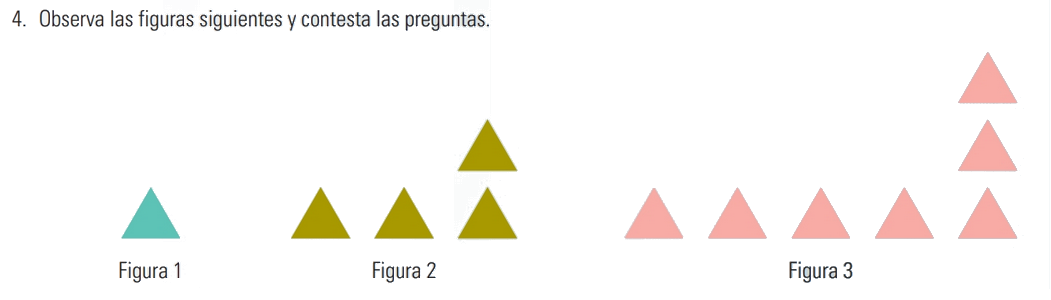
\includegraphics[scale=0.4]{p/i021.png} 
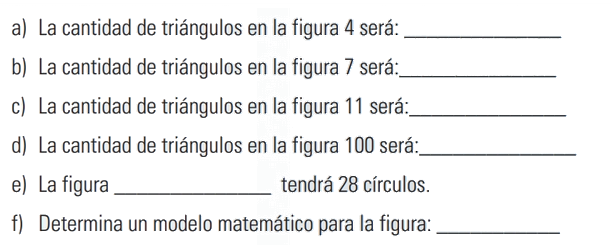
\includegraphics[scale=0.5]{p/i031.png} 

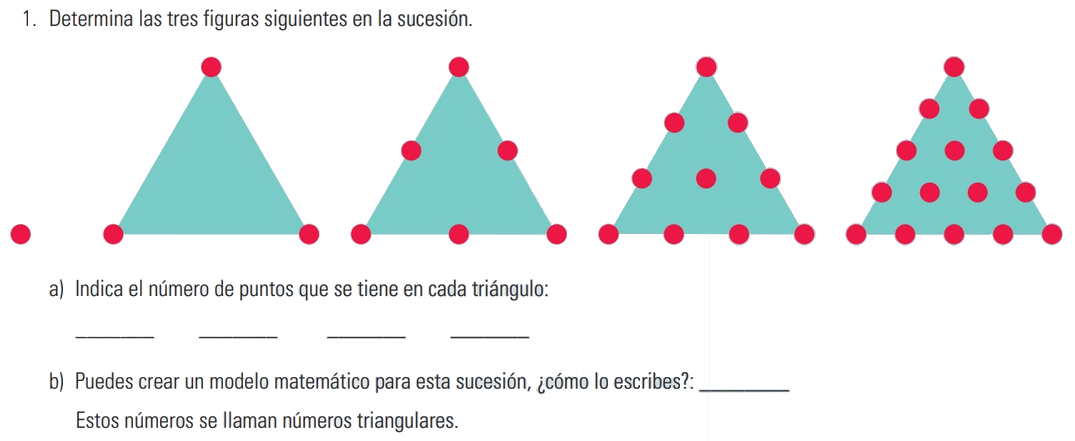
\includegraphics[scale=0.4]{p/i041.png} 
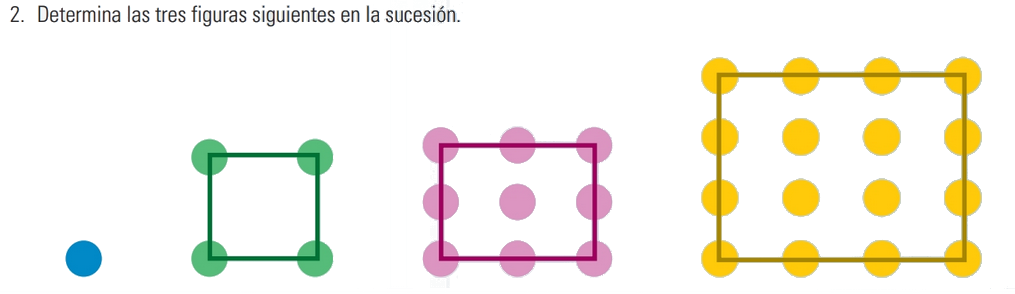
\includegraphics[scale=0.4]{p/i051.png} 

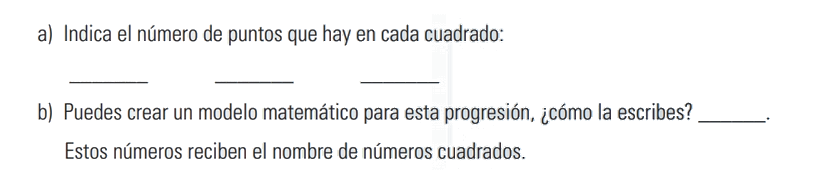
\includegraphics[scale=0.4]{p/i061.png} 

\vspace{\baselineskip}
% ex: ts=2 sw=2 sts=2 et filetype=tex
% SPDX-License-Identifier: CC-BY-SA-4.0

\question Una urna contiene canicas de colores: 10 son azules, 5 son
blancas, 12 son color café, 8 son doradas y 5 son color esmeralda. ¿Cuál es
la probabilidad de que al sacar una canica esta sea de color ...?

  \begin{tabular}{|l|c|c|l|l|l|}
    \hline
    \textbf{Evento} &  \textbf{Casos} & \textbf{Casos} &
    \textbf{Probabilidad} & \textbf{Decimal} &  \textbf{Porcentaje} \\
     &  \textbf{favorables} & \textbf{posibles} & & & \\
    \hline
    Azul & & & & & \\
    \hline
    Blanca & & & & & \\
    \hline
    Café & & & & & \\
    \hline
    Dorada & & & & & \\
    \hline
    Esmeralda & & & & & \\
    \hline
    \textbf{Suma} & & \textbf{Suma} & & & \\
    \hline
  \end{tabular}


\begin{EnvFullwidth}
  \sffamily\textbf{ Factoriza los trinomios siguientes.}
\end{EnvFullwidth}

% ex: ts=2 sw=2 sts=2 et filetype=tex
% SPDX-License-Identifier: CC-BY-SA-4.0

\question $x^2 + 8x + 16$

\vspace{\baselineskip}
% ex: ts=2 sw=2 sts=2 et filetype=tex
% SPDX-License-Identifier: CC-BY-SA-4.0

\question Resuelve las siguientes ecuaciones y compruebalos sustituyendo el
          valor de $x$

  \begin{parts}
    \part $6x+4 = 3x+10$ \\
    \\
    \\
    \\
    \part $6x+3 = 2x+11$ \\
    \\
    \\
    \\
    \part $2x+5 = x-3$
  \end{parts}

\vspace{\baselineskip}
% ex: ts=2 sw=2 sts=2 et filetype=tex
% SPDX-License-Identifier: CC-BY-SA-4.0

\question ¿Qué es una sucesión o progreción?
  \begin{solution}[2cm]
    Es un conjunto de números ordenados que siguen un patrón o regla
    especifica.
  \end{solution}

\vspace{\baselineskip}
% ex: ts=2 sw=2 sts=2 et filetype=tex
% SPDX-License-Identifier: CC-BY-SA-4.0

\question Una empresa exporta 10 toneladas de maiz y tiene una ganancia de
          \$25,000. ¿Cuánto será la ganancia si exporta 30 toneladas?

  \begin{solution}[2cm]
      $\frac{30 \times 25,000}{10} = 75,000$
  \end{solution}

\vspace{\baselineskip}
% ex: ts=2 sw=2 sts=2 et filetype=tex
% SPDX-License-Identifier: CC-BY-SA-4.0

\question ¿Qué tipos de sucesiónes hay?:
  \begin{solution}[2cm]
    Se clasifican en aritméticas, gemétricas, alfanuméricas y simbólicas
  \end{solution}

\vspace{\baselineskip}
% ex: ts=2 sw=2 sts=2 et filetype=tex
% SPDX-License-Identifier: CC-BY-SA-4.0

\question Sobre un cuerpo de $33$kg actua una fuerza de $297$\textbf{N}
          ¿Qué aceleración le proporciona dicha fuerza al cuerpo?

\makenonemptybox{1.6in}{Datos: \hspace{1cm} Formula: \hspace{1cm}
                      Despeje: \hspace{1cm} Sustitución y Resultado}

\vspace{\baselineskip}
% ex: ts=2 sw=2 sts=2 et filetype=tex
% SPDX-License-Identifier: CC-BY-SA-4.0

\question Dos magnitudes son inversamente proporcionales cuando al aumentar
          una, la otra disminuye en la misma proporción. A esto se le llama:
          \fillin[Proporcional inversa]

\vspace{\baselineskip}
% ex: ts=2 sw=2 sts=2 et filetype=tex
% SPDX-License-Identifier: CC-BY-SA-4.0

\question $x^2 - 9x + 8$


\vspace{\baselineskip}
% ex: ts=2 sw=2 sts=2 et filetype=tex
% SPDX-License-Identifier: CC-BY-SA-4.0

\question $c^2 + 5c - 24$


\vspace{\baselineskip}
% ex: ts=2 sw=2 sts=2 et filetype=tex
% SPDX-License-Identifier: CC-BY-SA-4.0

\question ¿Qué es rotación, traslación y percepción espacial?:

\vspace{\baselineskip}

\begin{EnvFullwidth}
  \sffamily\textbf{Analiza cada expresión y determina el valor de cada
  figura.}
\end{EnvFullwidth}

% ex: ts=2 sw=2 sts=2 et filetype=tex
% SPDX-License-Identifier: CC-BY-SA-4.0

\question 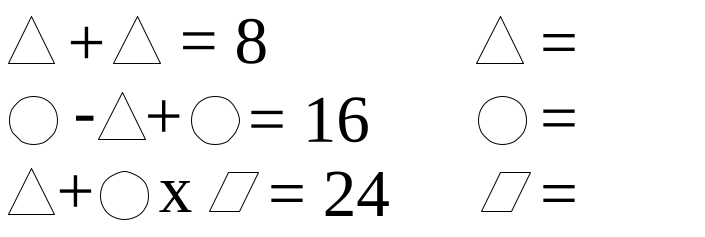
\includegraphics[scale=0.5]{p/i01.png}


\vspace{\baselineskip}

% ex: ts=2 sw=2 sts=2 et filetype=tex
% SPDX-License-Identifier: CC-BY-SA-4.0

\question 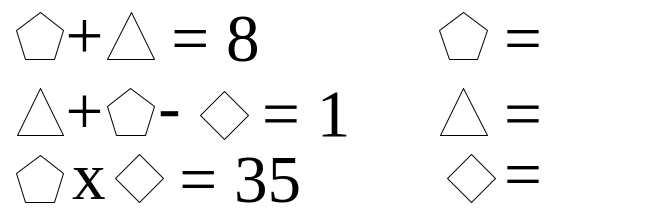
\includegraphics[scale=0.5]{p/i02.png}


\vspace{\baselineskip}

\end{questions}

\end{document}
